\section{Indledning} 

Verden er mere og tættere forbundet end nogensinde; men også mere
polariseret. Vi befinder os i en brydningstid, hvor der i
stigende grad savnes samfundsmæssig konsensus om et “facit”
om, hvordan verden arter sig og hvordan vi skal agere i den.  Vi
samles omkring forskellige konstellationer af verdensopfattelser,
for at opnå en fornemmelse af samhørighed blandt
meningsfæller \autocite{sulerUniqueGroupsCyberspace1999}.

Internettet gør det muligt, at finde dette fællesskab og denne
samhørighed på nye måder. Marginaliserede individer kan finde
sammen, upåagtet geografi, og deler frit og åbent erfaringer med
hinanden \autocite[s. 184]{sulerOnlineDisinhibitionEffect2004}. 
Der dannes positioner, hvor rettigheder, friheder, ansvar og
pligter forhandles i en evigt regenererende diskurs \autocite[s.
22]{harrePositioningTheoryMoral1999}.

Opleves der, at nogen siger det verdensbillede man har
internaliseret i mod, kan dette være megetsvært at acceptere.
Man oplever, at ens selvopfattelse og selvbillede krænkes. Den
position man har antaget bliver ikke altid anerkendt af andre,
eller at man ikke vil anerkende den position, andre forsøger at
placere en i \autocite[s 30]{harrePositioningTheoryMoral1999}.

De samme processer der gør, at mennesker kan tillade sig at være
mere sårbare og ærlige online, er også til grund for meget af
den grove tone man hurtigt finder på de sociale medier. Denne 
ondartede udgave af online disinhibition betyder, at der ikke skal
meget til, før miljøet online bliver giftigt
\autocite{sulerOnlineDisinhibitionEffect2004}.

Derudover har internettet bidraget med nye settings for at vise 
hvem man \sout{vil fremstå som at være} er. De sociale medier 
giver os nye rammer for sociale interaktioner, og nye scener for 
fremvisning af de roller vi identificerer os ved og ønsker at 
andre også genkender os i.

Jeg vil undersøge, hvordan disse processer arter sig på sociale
medier. Konkret vil jeg undersøge Instagram som præsentation- og
positionsarena, og se på hvordan selvpræsentationer bidrager til 
positionering omkring emnet maskulinitet.

Det følgende afsnit vil præsentere mit teoretiske grundlag for
denne undersøgelse. Derefter vil jeg introducere mit konkrete
fokusområde, med en efterfølgende kort gennemgang af undersøgelser
med et lignende fokus.

Herefter vil jeg drøfte mit empiriske analysegrundlag, med
tilhørende diskussion af mulige analyseresultater. Afslutningsvis
vil jeg diskutere og perspektivere mine konklusioner i et bredere
sociologisk perspektiv.

\section{Teoretisk analysegrundlag}

Jeg tager primært udgangspunkt i en positionsteoretisk tilgang, 
som beskrevet af \citeauthor{harrePositioningTheoryMoral1999}.   
Denne særlige, situerede diskursanalyse 
\autocite{harreRecentAdvancesPositioning2009} bliver suppleret med
bemærkninger fra 
\citeauthor{goffmanPresentationSelfEveryday1956}, hvor jeg 
anvender teatermetaforen præsenteret i 
\citetitle{goffmanPresentationSelfEveryday1956} 
(\citeyear{goffmanPresentationSelfEveryday1956}), på den 
formidling af “selv” der foregår på Instagram.  John Suler
bidrager med en cyberpsykologisk forståelse af, hvordan 
udbredelsen af cyberspace påvirker den menneskelige selvforståelse
og kommunikationsstrategi.

\subsection{Positioneringsteori}

\citeauthor{harrePositioningTheoryMoral1999} beskriver 
positioneringsteori som (\citeyear[s. 1, min oversættelse
]{harrePositioningTheoryMoral1999}):
\begin{quotation}
  \ldots studiet af lokale morale ordener som evigt skiftende 
  mønstre af gensidige og omtvistelige rettigheder og 
  obligationer af tale og handlen \ldots
\end{quotation}

Positioner påvirker således hvordan og hvorledes individuelle 
handlemåder og handlemuligheder arter sig. Er man positioneret som
uvidende om et emne, tildeles man ikke ret til at bidrage til 
diskussioner herom. Derudover er positioner generelt set
relationelle, idet at nogen må indtage positionen “magtesløs” for 
at andre kan have positionen “mægtig”.

Positioneringsteori vil undersøge, hvordan diskursive processer 
producerer psykologiske fænomener. Den tager udgangspunkt i, at 
vores oplevede liv brydes op i \emph{episoder} i gennem diskurser.  
Det er disse episoder, der er grundlaget for både vores
livshistorier og den sociale verden \autocite[s. 
4]{harrePositioningTheoryMoral1999}.

Episoder i denne kontekst omfatter “enhver serie hændelser hvor 
mennesker deltager, hvor der er en form for enhedprincip”. De 
indbefatter, ud over synlig adfærd, også deltagernes tanker, 
følelser, intentioner med mere. De både former deltagernes 
handlinger, og er definerede af dem \autocite[s. 
5]{harrePositioningTheoryMoral1999}.

Hvor en positioneringsteoretisk analyse adskiller sig fra for 
eksempel en interaktionsanalyse på baggrund af 
\citeauthor{goffmanPresentationSelfEveryday1956} i
\citetitle{goffmanPresentationSelfEveryday1956}, er et explicit 
fokus på situationens historicitet. Episoder bliver til på 
baggrund af foregående episoder, og vil indeholde elementer der 
ikke kan forklares på baggrund af generelle regler og roller 
\autocite[s. 5-6]{harrePositioningTheoryMoral1999}.

Dermed fremhæves tre grundlæggende egenskaber af, hvordan sociale 
og psykiske fænomener konstrueres 
\autocite{harrePositioningTheoryMoral1999}:
\begin{enumerate}
  \item
    deltagernes morale positioner, og tilhørende ret og pligt 
    til bestemte ytringer
  \item
    samtalens historik
  \item
    de faktiske udsagn, med kraft til at give form til dele af 
    den sociale verden
\end{enumerate}

\subsubsection{Positioneringens forståelsesramme}

Indenfor positioneringsteorien anses mennesker for, at være fokus 
for sociale handlinger, hvor “samtalen” er den grundlæggende 
bestanddel af den sociale verden. Der er i samtalen,
den sociale verden bliver skabt; og sociale handlinger genereres 
og reproduceres \autocite[s. 
15]{harrePositioningTheoryMoral1999}.

I denne forståelse af den sociale verden som bestående af 
\emph{personer} og \emph{samtaler}, er positionering en “\ldots 
diskursiv konstruktion af personlige fortællinger, der gør en 
persons handlinger forståelige og relativt fastgjorte som sociale 
handlinger, og hvori samtalens medlemmer har specifikke 
placeringer.” \autocite[s. 16]{harrePositioningTheoryMoral1999}

Dermed er positioner i en samtale en samling af personens moralske
og personlige egenskaber. Man kan positionere sig — eller blive 
positioneret — som mægtig eller magtesløs, selvsikker eller 
undskyldende, med videre. En handlings sociale gennemslagskraft og
deltagernes positioner er videre forbundne, idet samtaler har 
historier, og de positioner der indtages i en samtale er forbundne
med disse historier. Der er dermed en gensdigt skabende triade, 
bestående af følgende elementer \autocite[s.  
17-18]{harrePositioningTheoryMoral1999}:


\begin{figure}[!h]
\label{fig:triad}
\centerline{
  % Resize it to 5cm wide.
  \resizebox{7cm}{!}{
    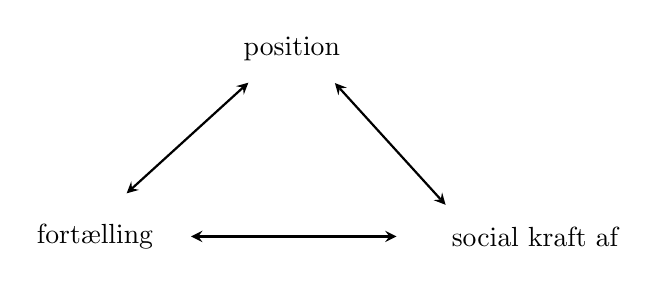
\begin{tikzpicture}[
      scale=0.5,
      trans/.style={thick,<->,shorten >=2pt,shorten 
      <=2pt,>=stealth},
    ]
    \draw[trans] node {fortælling} (0.7,1) -- (4,4) node[above, 
    xshift=0.5cm, yshift=0.1cm] {position};
    \draw[trans] (6,4) -- (9,0.7);
    \draw[trans] (2.3,0) -- (7.8,0) node[right, xshift=0.5cm] 
  {social kraft af}; \end{tikzpicture}
  }
}
\caption{De tre gensidigt afhængige elementer i en situation}
\end{figure}


Positioner kan opstå “naturligt” i situationen; men en besiddelse 
af den dominerende rolle i en samtale vil kunne tvinge de andre 
talere i positioner de ellers ikke ville have indgået frivilligt. 
Dog kan disse begyndende positioner anfægtes, og talerne dermed 
blive ompositionerede \autocite[s. 
18]{harrePositioningTheoryMoral1999}. Disse “naturligt” 
forefindende positioner er selv produkter af  positionshandlinger
af højere ordener, hvor rettigheder og  pligter til at tillægge
eller modstå positioner distribueres  \autocite[s.  
8]{harreRecentAdvancesPositioning2009}.

Ved at starte en samtale af en højere orden, hvor den foregående 
samtale blot er et emne, kan man positionere sig som kommentator 
på positioner, historier og sociale handlinger deri \autocite[s.  
18]{harrePositioningTheoryMoral1999}. Videre kan den samme 
historie være del i flere narrativer der foregår sideløbende, og
have forskellige  betydninger i hvert narrativ 
\autocite{harreRecentAdvancesPositioning2009}.

Positioneringsteorien ser dermed på hvordan mennesker opfører sig 
overfor hinanden, og forsøger at afdække de implicitte og 
eksplicitte tankemønstre der ligger til grund for dette 
\autocite[s. 5]{harreRecentAdvancesPositioning2009}.
Fokus er dermed ikke på et direkte kausalitetforhold mellem social 
handlinger; men derimod på de meningsforhold der forbinder dem.  
Disse meningsforhold springer ud af en lokal kanon af normer og 
regler, og er også med til, at mediere forholdet mellem bærere af 
specifikke medier \autocite[s. 
7]{harreRecentAdvancesPositioning2009}.

\subsection{Selvets præsentation}

I den førnævnte \citetitle{goffmanPresentationSelfEveryday1956} 
beskriver \citeauthor{goffmanPresentationSelfEveryday1956} hvordan 
mennesker præsenterer forskellige facetter af sig selv i 
forskellige sammenhænge. “Selvet” er i denne forståelse 
relationelt, og er afhængigt af, at de personer individet 
interagerer med i en given situation anerkender den \emph{persona} 
individet har antaget denne situation, og dermed også individets 
moralske ret til at blive behandlet på en bestemt måde 
\autocite[s.  6-7]{goffmanPresentationSelfEveryday1956}.

\citeauthor{goffmanPresentationSelfEveryday1956} anvender en 
teatermetafor gennemgående i sin analyse. De forskellige personaer 
bliver i denne sammenhæng kaldt \emph{roller}, og de andre 
deltagere i en situation (hvad i en positionsanalyse vil være en 
episode) bliver tilskuere til en præsentation. Samtidig spiller 
disse tilskuere selv en rolle, og vi er på denne måde alle 
hinandens tilskuere 
\autocite[forordet]{goffmanPresentationSelfEveryday1956}.

Dette relationelle selv individet præsenterer vil, i følge 
\citeauthor{goffmanPresentationSelfEveryday1956} være et 
idealiseret selv. Individet vil ikke være i besiddelse af alle de 
kvaliteter, der er forventet af rollen, men forsøger at leve op 
til disse alligevel (\citeyear[s.  
?]{goffmanPresentationSelfEveryday1956}). Individet vil dermed 
forsøge konstant at bedrive “impression management”, for at 
henlede opmærksomheden væk fra de områder hvor det ikke er 
opnåeligt, at leve op til rollens krav. Samtidig vil tilskuerne 
anvende pli og høflighed, for ikke at gøre opmærksom på, at der er 
sket et fejltrin \autocite[s.  
7-8]{goffmanPresentationSelfEveryday1956}.

For at kunne opretholde en social front, taler 
\citeauthor{goffmanPresentationSelfEveryday1956} om 
\emph{settings}, der udgør den scenografiske del af en optræden, 
samt \emph{udseende} (der giver os indblik i individets sociale 
status) og \emph{opførsel} (der kan fortælle os, hvilken rolle 
individet forventer at indtage).  Der er ofte en forventning om, 
at der er et vist samsvar mellem setting, udseende og opførsel 
\autocite[s. 14-15]{goffmanPresentationSelfEveryday1956}.

Optrædener foregår gerne i en afgrænset \emph{region}, og kaldes 
af \citeauthor{goffmanPresentationSelfEveryday1956} \emph{front
region}. Der foretages en analytisk sondring mellem  denne
frontregion, hvor rollen udleves; og regionen  \emph{backstage},
hvor rollen kan lægges væk, og individet kan få  afløb for de
sider af sig selv, der ikke er forenelig med rollen  (\citeyear[s.
69]{goffmanPresentationSelfEveryday1956}).

\section{Instagram som positionerings- og præsentationsarena}

Instagram er et socialt medie bygget op omkring offentliggørelse 
af billeder og korte videoklip\footnote{Der er dog mulighed for,
at opretholde en privat profil på Instagram, hvor man skal 
godkendes som følger af en bruger for at se vedkommendes 
billeder.}. Medlemmer kan “følge” andre brugere, for at inddrage 
disse brugeres opslag i den strøm af billeder, der møder en når 
man åbner appen. De publicerede billeder kan suppleres med en
billedtekst, der ofte indeholder 
\texttt{\#hashtags}.  Disse hashtags samler flere billeder omkring
et emne — til en samtale, om man vil. Hashtags gør det også muligt
for billeder at nå frem til andre der er interesserede i samme 
emne, uden at disse brugere aktivt følger personen, der lagde 
billedet op. Dette kan både ske aktivt; ved at følge et bestemt
hashtag, eller passivt; ved at Instagrams algoritmer foreslår
opslag.

Når det sociale ses som bestående af personer og samtaler, er der 
her mange samtidige samtaler at gribe fat i med et 
positioneringsteoretisk blik. Selve billedet er et bidrag til en 
samtale. Derudover er billedtekst og tilhørende hashtags med til, 
at vise hvilken position der indtages omkring et bestemt emne — 
og, qua den iboende relationelle kvalitet i positioneringen, 
hvilke positioner der konstrueres for ens “modstandere” omkring 
dette emne. Og billedteksten er at regne for en social ytring — 
der har (potentiel) kraft til at forme den sociale verden.

Men den sociale positionering er ikke kun indbefattet i den 
konkrete ytring. Udvælgelse af hashtags, og de fællesskaber man 
dermed henvender sig til og (dis)associerer sig med, er også en 
form for social talehandling. Den vil også påvirke og forholde sig 
til en social fortælling — og ikke nødvendigvis den samme, som 
billede og billedtekst.

Det er her vigtigt, at holde sig for øje, at en talehandling kan 
yde indflydelse på to måder: hvad der opnås, \emph{i at sige 
noget}, og og hvad der opnås \emph{ved at sige noget} \autocite[s.
17]{harrePositioningTheoryMoral1999}. Dermed bliver udsagnet “Hvor
blev de rigtige mænd af?” både en kommentar til de skiftende 
holdninger til maskulinitet, og en tilkendegivelse af egne 
holdninger.

\subsection{Selvudstillelse eller selvskabelse?}

Havde man spurgt \citeauthor{goffmanPresentationSelfEveryday1956} 
om hans holdning til ovenstående spørgsmål, ville han formentlig 
kigget uforstående tilbage. For ham var de to ting uløseligt 
sammenbundne. Ved at udstille sig som det “selv” individet ønsker 
at fremstå som, skaber individet en opfattelse af sig som dette 
“selv”.

Instagram er, i teatermetaforen, en en særlig form for performativ 
scene, hvor man har gode muligheder for at styre andres 
opfattelser af en selv. Det er muligt, at holde en skarp 
adskillelse af front- og backstage, hvor det online publikum ikke 
får adgang til rollens konstruktion. Individet har videre god 
kontrol over de sceniske aspekter af sin optræden, og kan styre de 
sociale tegn der formidles igennem rekvisitter med videre. 

En af de mest fremtrædende forskere i sociale mediers betydning
for individer er den amerikanske psykoanalytiker John Suler. 
\citeauthor{sulerSelfPortraitsSelfies2015} har set på, hvordan 
mennesker iscenesætter sig selv online via selvportrætter — 
“selfies”. Instagram består ikke kun af selfies. Men den generelle 
idé, der peges på, kan overføres til andre billeder der 
distribueres på sociale medier som en del af selv-præsentation og
kontrol af andres indtryk af ens (aktuelle) selv. Det er en
effektiv måde, at løfte sløret for sig “selv”, samtidig med, at
man forsøger at styre denne fremvisning af selvet 
(\citeyear{sulerSelfPortraitsSelfies2015}).

På Instagram kan andre brugere give ens opslag et “like”, hvor der 
tilkendegives en form for abstrakt anerkendelse af, den ytring og 
optræden der er blevet udført. Dette “like” er dermed også en form 
for talehandling, der anerkender rollen og accepterer positionen 
der indtages ved opslaget.

\citeauthor{sulerSelfPortraitsSelfies2015} nævner dog, at dette 
har en følgevirkning — der kan opstå en selektiv effekt af 
respons. Man udvælger de billeder der bliver lagt op, på baggrund 
af hvor mange likes og kommentarer de kan afstedkomme.  Her kan 
dele af ens identitet og livsoplevelser blive underkendt, og 
individet risikerer at føle sig fastlåst i en bestemt 
selvopfattelse (\citeyear{sulerSelfPortraitsSelfies2015}).

\citeauthor{goffmanPresentationSelfEveryday1956} beskrev noget 
(næsten) ubevidst i hans samtid. De sociale medier gør det mere 
bevidst for den enkelte, at man aktivt konstruerer sig selv.
Det observerende ego er blevet selv-fortæller i sin egen 
(livs)historie \autocite{sulerSelfPortraitsSelfies2015}.

\subsection{Online kommunikation og manglende hæmninger}

I \citetitle{sulerOnlineDisinhibitionEffect2004} beskriver 
\citeauthor{sulerOnlineDisinhibitionEffect2004}  en række 
forklarende årsager til, at man slipper sine
hæmninger online (\citeyear{sulerOnlineDisinhibitionEffect2004}).

Her vil jeg fremhæve \emph{disassociativ anonymitet} — “jeg” på de
sociale medier er en anden end “jeg” i den analoge verden.  Dermed
skal det analoge “jeg” ikke stå til ansvar for, hvad det online 
“jeg” foretager mig. Tæt beslægtet er den disassociative fantasi — 
den online verden er en anden verden, uafhængig af den udenfor.
Den indirekte, asynkrone kontakt gør endvidere den anden “usynlig”
for en — man undgår øjenkontakt, og kan flygte fra åstedet uden at
skulle stå til direkte ansvar for sin udlevering \autocite[s.  
184]{sulerOnlineDisinhibitionEffect2004}.

Suler skelner mellem en godartet og en ondartet udgave af denne
disinhibitionseffekt. Når man taler om uhensigtsmæssig opførsel
online, er det primært det sidste, der tales om; kendetegnet af
vrede, had, og vold. Den godartede er kendetegnet ved, en form for
bearbejdning og øget forståelse af sig selv, ifølge Suler, hvor
den ondartede blot er destruktiv udtømning \autocite[s.  
185]{sulerOnlineDisinhibitionEffect2004}.

\section{Fokusområde}

Den 13.\ januar 2019 offentliggjorde  
\citeauthor{gilletteWeBelieveBest2019} en reklame på YouTube, der
i det første minut udlægger eksempler på en særlig stereotypi af
mandlig opførsel. Mænd lægger ord i kvinders mund, står og kigger
på drenge der slås (\textit{“det er blot drengestrege”}), opfører 
sig seksuelt upassende overfor kvinder, mobber og driller.

Indtil der sker noget. I hvert tilfælde er der nogen der tager
affære — stopper en kammerat fra at fløjte efter en pige; griber
ind i slåskampen; jager mobberene væk. Altid er der unge drenge
der kigger på.

Budskabet virker svært at tage fejl af. Dagens unge drenge kigger
på os mænd, for at lære hvordan de skal opføre sig når de engang
bliver mænd selv. Dette gøres overtydeligt klart i videoen: 
\textit{“The boys of today will be the men of tomorrow”}.

Med andre ord: Vi socialiseres (blandt andet) efter eksempler. Ved
at justere vores eksempler, kan vi ændre på udfaldet af
socialisering.

Der kom dog en kraftig modreaktion fra (primært) mænd.
Den pågældende adfærd blev ikke set som et “problem” der skulle
“løses”, endsige noget at undskylde for. Gillette blev
beskyldt for, at ville udslette mænd og mandighed, og der blev
opfordret til, at boykotte Gillettes skrabere og barberblade 
\autocite{nashGilletteFacesWidespread2019}. Videoen blev hurtigt 
mødt med “dislikes”, og er i skrivende stund på næsten halvanden 
million nedadvendte tomler, og nummer 24 på listen over videoer på 
YouTube med flest dislikes 
\autocite{wikipediaListMostdislikedYouTube2019}.

Der kom (forventeligt) en reaktion på modreaktionen; hvor blandt 
andet det, at nogle ikke kunne genkende denne form for 
maskulinitet som noget “forkert” blev fremstillet som bevis for
nødvendigheden af dette budskab 
\autocite{mutherBacklashGilletteAd2019}. 

Som ridset op ovenfor, viser reaktionerne på reklamen forskellige
perspektiver og forståelser af begreberne “mandighed” og
“maskulinitet”. Disse positioner, om man vil, ser jeg som ydre
tegn på socialiseringprocesser og socialiseringsudfald. 

De sociale medier udgjorde en arena, hvor denne kamp for 
definitionsret udspillede sig. Jeg vender blikket til Instagram, 
og ser på, hvordan menneskers selvpræsentation bidrager til disse 
positioneringsprocesser.

\subsection{I videnskabelig dialog}

% FIXME: Needs a better throughline
%        And more maybe?
I forhold til positioneringsteori, online kommunikation og 
identitetsdannelse, har bl.a 
\citeauthor{lopezlongTweetingChoirReligious2012} set på, hvordan 
individers positionerer sig og grupper de er associeret med på 
Twitter (\citeyear{lopezlongTweetingChoirReligious2012}); og 
\citeauthor{dennenFacilitatorPresenceIdentity2011} har med held 
anvendt positioneringsteori til at analysere asynkron, online 
kommunikation (\citeyear{dennenFacilitatorPresenceIdentity2011}).

Jeg er langt fra den første, der bruger Goffmans analytiske 
redskaber og begreber i en analyse af den særlige setting vi ser 
på de sociale medier. Det er blevet undersøgt, hvordan unge 
mennesker ser på sin aktive selvkonstruktion på Instagram 
\autocite{seehaferNOFILTERExplorationInstagram2017a}, og hvordan 
man aktivt viser, at man køber ind på et særligt syn på køn og 
kønsroller \autocite{bakerGoodMorningFitfam2018}.

Der er også foretaget en analyse af selfies på Instagram, der er 
blevet fordelt over en række genrer 
\autocite{eagarClassifyingNarratedSelfie2016}. Her bruges der også 
en narrativ metafor, i forståelsen af personlig histore der 
underbygger individets personlige “brand”. Brug
af Instagram til selvkonstruktion og selvpræsentation undersøges 
af \citeauthor{lazebnaRoleCommunicationApprehension2015}, dog med 
et udgangspunkt i et “autentisk selv” 
(\citeyear{lazebnaRoleCommunicationApprehension2015}).

\citeauthor{parentSocialMediaBehavior2018} antyder, at toksisk 
maskulinitet (karakteriseret af et behov for at dominere andre, 
samt misogynistiske og homofobiske holdninger) kan være 
selvforstærkende i, at fremme depressivitet hos mænd. Dette øger i 
igen sandsynligheden for overt toksisk maskulin adfærd online 
\autocite{parentSocialMediaBehavior2018}. Sammenholdt med den 
online disinhibition, er dette en yderligere forklaring på, 
hvorfor nogle individer og nogle fora online er meget ubehagelige 
at overvære.

\subsubsection{Mit bidrag til den videnskabelige dialog}

Med positioneringsteorien som udgangspunkt for en diskursiv 
analyse, håber jeg at vise, hvordan indlejrede “selvfølgeligheder” 
i vores forståelsesrammer bidrager til vores forståelse og 
behandling af andre mennesker i den sociale verden. Jeg ser på 
hvordan disse selvfølgeligheder formidles og genskabes gennem den 
særlige form for social interaktion der kendetegner de sociale 
medier.

Jeg indskriver mig i en socialkonstruktionistisk videnstradition, 
der ser den sociale verden som konstrueret af meninger og 
betydninger mellem aktører. Ved at belyse, hvordan synet på køn og 
kønsroller er socialt medieret, kan jeg bidrage til en øget 
forståelse af identitetsdannelse og selvpræsentation i en 
hyperforbundet verden.

\section{Undersøgelsesdesign}

Jeg ser på udvalgte samtaler omkring maskulinitet på Instagram i
kølvandet af reklamen Gillette offentliggjorde 13.\ januar 2019.  

Denne positioneringsteoretiske tilgang vil blive suppleret med
interaktionsanalytiske begreber, idet Instagram også kan ses som 
en del af etableringen af et individs selvfortælling via 
selviscenesættelse. 

For at finde opslag på Instagram, der lægger sig klart i hver af 
de to lejre beskrevet ovenfor, trækker jeg de opslag ud, hvor så 
mange som muligt af nogle udvalgte hashtags fremgår. Ud fra disse 
billeder, udvælger jeg et opslag under hvert hashtag, jeg mener 
giver grundlag for en god analyse.

\subsection{Forskningsspørgsmål}

Hvordan viser positioneringer
omkring maskulinitet sig? Hvem positionerer hvem? Hvem modsætter
sig disse positioneringer? Er der bestemte identiteter, der søges
forsvaret eller etableret ved at indtage bestemte positioner?
Medieres positionsprocesserne af tendensen til online
disinhibition?

\subsection{Empirisk analysegrundlag}
%\input{../fig/tag_table}
For at kortlægge de forskellige positioner omkring denne 
diskussion af maskulinitet starter jeg med at lave en optælling af 
hashtags på Instagram.

De hashtags jeg kigger på er:
\begin{itemize}
    \item
        \texttt{\#thebestmencanbe}
    \item
        \texttt{\#boycottgillette}
    \item
        \texttt{\#gillettead}
\end{itemize}
\texttt{\#thebestmencanbe} er Gillettes nye slogan; og er som 
sådan samlende for den generelle diskussion omkring reklamen.  
Dette er også gældende for \texttt{\#gillettead}.  
\texttt{\#boycottgillette} er derimod udtryk for en mere kritisk 
holdning til varemærket.

Inden jeg tæller op, foretager jeg dog nogle databehandlingsgreb 
\footnote{Mit datagrundlag er offentligt tilgængeligt på GitHub 
\autocite{andersenEksamensopgaveSocialiseringOg2019}}:
\begin{itemize}
  \item
        al tekst bliver gjort om til kun at bestå af små bogstaver
    \item
        jeg begrænser mig til opslag fra 13.\ januar 2019 indtil, 
        givetvis lidt tilfældigt, 8.\ april 2019
      \item
        Da jeg har hentet Instagram opslag under specifikke 
        hashtags hver for sig, har jeg øje for at undgå dupletter 
        ved den samlede optælling.
    \item
        Jeg kigger kun på opslag, hvor de pågældende hashtags 
        indgår i billedteksten. Opslagene under de forskellige 
        hashtags hvor hashtagget kun fremgik af kommentarerne er 
        dermed ikke medtaget.
\end{itemize}

\subsection{Metodologiske begrænsninger}

Jeg har haft fokus på det enkelte opslag på Instagram. Instagram 
som socialt medie har ikke en funktion, som mange andre sociale 
medier har: muligheden for, at dele andres opslag (hvad der på 
Twitter og Facebook vil være et “retweet” eller et “share”).  
Dermed kan der laves mere sofistikerede kortlægninger over 
fænomener og menneskers engagement i dem end jeg har haft mulighed 
for.

Jeg ser i denne udlægning primært Instagram som et billedligt 
medie, med fokus på det enkelte billedes performativitet. Som jeg 
nævnte ovenfor, er det også muligt, at publicere korte videoklip 
på Instagram; og man kan også have op til ti billeder i et opslag, 
der præsenteres sekventielt. De analytiske redskaber ovenfor er 
lige så anvendelige på denne form for opslag, om end jeg ikke har 
medtaget dette perspektiv.

Jeg har også kun udvalgt offentlige opslag, og ikke såkaldte 
“stories”, der kun er tilgængelige i 24 timer. Dog er det muligt, 
at holde samlinger af “stories” fastgjort til sin profil, hvilket 
også har performative og positioneringsmæssige aspekter. Dette 
falder udenfor denne opgaves remis.

Jeg har set på den pågående samtale omkring maskulinitet som 
helhed, og har dermed ikke set på samtalens udvikling over tid — 
er der særlige hashtags eller beskrivelser der vinder frem omkring 
emnet, for eksempel? Jeg har også kun set efter hashtags i 
billedtekster, og har dermed ikke fanget de opslag, hvor hashtags 
ikke indgår, eller hvor hashtags fremgår i en kommentar til 
opslaget. En større netværksanalyse af hashtags indbyrdes forhold 
foretager jeg mig heller ikke.

\section{(Skitsen af) en analyse}

\begin{table}[H]
    \footnotesize
    \caption{De hyppigste hashtags }
    \begin{subtable}{.25\linewidth}
\centering
\captionsetup{justification=centering,singlelinecheck=off}
\caption{
  Hele datasettet
}
\begin{tabular}{lr}

\texttt{\#thebestmencanbe}  & 971 \\
\texttt{\#gillette}         & 942 \\
\texttt{\#gillettead}       & 757 \\
\texttt{\#boycottgillette}  & 565 \\
\texttt{\#toxicmasculinity} & 531 \\
\texttt{\#metoo}            & 329 \\
\texttt{\#feminism}         & 213 \\
\texttt{\#masculinity}      & 209 \\
\texttt{\#men}              & 206 \\
\texttt{\#feminist}         & 159 \\

\end{tabular}
    \end{subtable}%
    \begin{subtable}{.25\linewidth}
\centering
\captionsetup{justification=centering,singlelinecheck=off}
\caption{
  \texttt{\#thebestmencanbe}
}
\begin{tabular}{lr}
\texttt{\#thebestmencanbe}   & 972 \\
\texttt{\#gillette}          & 382 \\
\texttt{\#metoo}             & 206 \\
\texttt{\#toxicmasculinity}  & 191 \\
\texttt{\#repost}            & 132 \\
\texttt{\#men}               & 85 \\
\texttt{\#masculinity}       & 76 \\
\texttt{\#feminism}          & 67 \\
\texttt{\#gillettead}        & 63 \\
\texttt{\#feminist}          & 57 \\

\end{tabular}
    \end{subtable}%
    \begin{subtable}{.25\linewidth}
\centering
\captionsetup{justification=centering,singlelinecheck=off}
\caption{
  \texttt{\#gillettead}
}
\begin{tabular}{lr}

\texttt{\#gillettead}         & 755 \\
\texttt{\#gillette}           & 442 \\
\texttt{\#toxicmasculinity}   & 270 \\
\texttt{\#metoo}              & 122 \\
\texttt{\#feminism}           & 117 \\
\texttt{\#masculinity}        & 99 \\
\texttt{\#men}                & 89 \\
\texttt{\#feminist}           & 84 \\
\texttt{\#gillettecommercial} & 69 \\
\texttt{\#thebestmencanbe}    & 62

\end{tabular}
    \end{subtable}%
    \begin{subtable}{.25\linewidth}
\centering
\captionsetup{justification=centering,singlelinecheck=off}
\caption{
  \texttt{\#boycottgillette}
}
\begin{tabular}{lr}

\texttt{\#boycottgillette}   & 564 \\
\texttt{\#gillette}          & 204 \\
\texttt{\#toxicmasculinity}  & 125 \\
\texttt{\#maga}              & 110 \\
\texttt{\#buildthewall}      & 101 \\
\texttt{\#trump2020}         & 74 \\
\texttt{\#trumptrain}        & 66 \\
\texttt{\#agentprovocateurs} & 61 \\
\texttt{\#berniesanders}     & 60 \\
\texttt{\#falseflag}         & 59

\end{tabular}
    \end{subtable}
\end{table}


Ser man på datagrundlaget samlet, og tæller alle indslag der har 
mindst 1 af de ovennævnte hashtags, er der, ud over disse, klar 
overvægt af \texttt{\#gillette}, med \texttt{\#feminism} 
\texttt{\#metoo} og \texttt{\#toxicmasculinity} efterfølgende

At \texttt{\#toxicmasculinity} er med på en femteplads, er i
fin tråd med, at Gillette skriver sig ind i en diskussion omkring
et skiftende syn på maskulinitet.

Ser man på de mest populære hashtags forbundet med
\texttt{\#thebestmencanbe}, figurerer  \texttt{\#metoo} på en
tredjeplads, over \texttt{\#toxicmasculinity}.  Noget 
bemærkelsesværdigt er det, at \texttt{\#repost} lige er med på en
femteplads, idet Instagram ikke har en indbygget funktionalitet
til, at gengive eller forstærke en anden brugers opslag.

Ved \texttt{\#gillettead} er de fleste hashtags sammenfaldende med 
\texttt{\#thebestmencanbe}. Hashtags som \texttt{\#feminism}, 
\texttt{\#men} og \texttt{\#masculinity} er på begge lister. Noget 
slående forekommer de to ovenstående hashtags dog sjældent 
samtidigt.

En frekvenstabel over de mere kritiske opslag, hvor der opfordres 
til boykot af Gillette, viser at \texttt{\#toxicmasculinity} igen 
er med, med \texttt{\#maga} og andre Trump-sympatiske hashtags 
umiddelbart derefter. Der er ingen hashtags med der sætter 
reklamevideoen i et større perspektiv, som ved de to første 
lister.

\subsection{Udvælgelse af opslag til analyse}

Jeg søger nu i mine indsamlede opslag fra Instagram, for at finde 
opslag i hver generelle gruppering. Jeg ser efter opslag, hvor 
flere af de mest hyppige hashtags forekommer samtidigt i
billedteksten.

\subsubsection{\texttt{\#thebestmencanbe}}

Ved \texttt{\#thebestmencanbe} var jeg nødsaget til, at stoppe 
efter \texttt{\#toxicmasculinity}. Ved inklusion af 
\texttt{\#repost}, kom der ingen resultater frem.  det var også 
ved denne hashtag jeg blev nødt til at stoppe ved 
\texttt{\#boycottgillette}, for at have et stort nok grundlag at 
vælge ud fra. 

En del af opslagene herunder var henvisninger til YouTube, blogs 
eller nyhedsmedier hvor man kunne finde brugerens kommentarer.  
Her gerne med et screenshot af videoen som billedmateriale. Langt 
de fleste andre var billeder af tekst, der kommenterede på emnet.  
Der var dog også opslag som det vist her, der viser og fortæller 
en personlig historie:

\begin{figure}[H]
    \footnotesize
    \centering
    \begin{subfigure}[b]{0.48\linewidth}
        \includegraphics[width=\textwidth]{../data/cases/thebest/2019-01-17_22-24-27_UTC.jpg}
    \end{subfigure}
    \qquad
    \begin{subfigure}[b]{0.3\linewidth}

        Me rolling my eyes at all the a n g e r y menfolk after 
        they watched the Anti Toxic Masculinity Gillette advert.
        Why don’t you just smile? You’d be much prettier if you 
        smiled.
        % 🔥

        My narcissist ex was like that, convinced that he was 
        superior to women in every way and full of the “boys will 
        be boys” rhetoric that society has absorbed and 
        perpetuated for so long. I’m working up to a series of 
        posts about \#narcissisticabuse and \#dvsurvival, and 
        there will be appropriate CWs when I do.  Happy Thursday, 
        friends and followers % 🧡

        \#toxicmasculinity \#toxicmasculinityruinsthepartyagain 
        \#toxicrelationships \#mentalhealthawareness 
        \#mentalhealth \#gillette \#metoo \#cptsdrecovery \#cptsd 
        \#mentalillness \#recovery \#redhead \#redhair \#curlyhair 
        \#curls \#verylonghair \#makeup \#eyebrows \#goth 
        \#freckles \#eyeroll \#naturalredhead 
        \#domesticviolenceawareness \#domesticviolence 
        \#invisibleillness \#thebestmencanbe
    \end{subfigure}
    \caption{@\citeauthor{rebelliousredhead2019} på Instagram}
    \label{img:thebest}
\end{figure}


\subsubsection{\texttt{\#gillettead}}

Om \texttt{\#gillettead} var det mindre spredning af hashtags på 
individuelle opslag. Jeg fik et fint grundlag at vælge fra med 
inklusion af hashtags frem til og med \texttt{\#feminism}. Næsten 
alle opslag i denne pulje var af typen billede-af-tekst; men ikke 
nødvendigvis tekst forfattet af brugeren selv, som eksempelet 
herunder viser:

\begin{figure}[H]
    \footnotesize
    \centering
    \begin{subfigure}[b]{0.48\linewidth}
        \includegraphics[width=\textwidth]{../data/cases/ad/2019-01-17_12-32-22_utc.jpg}
    \end{subfigure}
    \qquad
    \begin{subfigure}[b]{0.3\linewidth}

    \#gilletteadvert \#gillette \#toxicmasculinity 
    \#notforsensitiveskin \#insecure \#sexualharassment 
    \#sexualassault \#rapeculture \#metoo \#bethebestmanyoucanbe 
    \#feminist \#feminism \#speakup \#calloutyourbros 
    \#thebestamancanget \#woke \#thismakesmehappy \#gillettead

    \end{subfigure}
    \caption{@\citeauthor{elle_sciencekitty2019} på Instagram}
    \label{img:ad}
\end{figure}


\subsubsection{\texttt{\#boycottgillette}}

Ved \texttt{\#boycottgillette} var jeg nødt til, kun at forholde 
mig til de tre øverste hashtags, da mit datagrundlag ellers ville 
blive for snævert. Også her var der mange eksterne links og 
billeder af tekst; men der var også i højere grad anvendt såkaldte 
“memes” og “image macros” som en måde, at kreativt bidrage til 
debatten.

Der var til gengæld også langt flere personlige opslag, hvor 
brugeren figurerede i billedet, så som følgende:

\begin{figure}[H]
    \footnotesize
    \centering
    \begin{subfigure}[b]{0.48\linewidth}
        \includegraphics[width=\textwidth]{../data/cases/boycott/2019-01-18_18-43-33_UTC.jpg}
    \end{subfigure}
    \qquad
    \begin{subfigure}[b]{0.3\linewidth}

        I never boycott products, but I am now.. \@gillette went 
        in the trash this morning right after I saw their new add.  
        I am proud of being a man and will nor should ever be 
        ashamed of that.  We are half of the entire world Gillette 
        and your entire customer base.

        Never using their products again.  Who can recommend a 
        good alternative razor?

        I'll join others in pledging a \$100 purchase to any razor 
        company that puts out a counter ad.  I'll also post their 
        product on here.
        
        \#gillette \#thebestamancanget \#toxicmasculinity 
        \#masculinity \#razor \#shaving \#shave \#boycottgillette 
        \#boycott \#metoo \#trash \#man \#men \#male \#shavingcream 
        \#razorblade \#gillette \#picoftheday \#friday 
    \@dollarshaveclub \@harrys \@bevel \@theartofshaving    
\end{subfigure}
    \caption{@\citeauthor{david_s1000rr2019} på Instagram}
    \label{img:boycott}
\end{figure}


\section{Afrunding}

\subsection{Tentative konklusioner}

Frekvenstabellerne over de hyppigst forekomne hashtags forbundet 
med mine udvalgte hashtags giver et billede af, de mange samtidige 
samtaler der foregår omkring “maskulinitet”. Mest påfaldende er 
\texttt{\#boycottgillette}, hvor kun to hashtags også figurerer i 
de andre to lister.

De mange samtaler viser også, at man positionerer sig i 
samhørighed til andre. Det selv der præsenteres, vil dermed formes 
af og tilpasses den gruppeidentitet man (mere eller mindre 
ubevidst) ønsker at projicere. Man tager standpunkter og 
positioner, hvorfra man (\emph{i den pågældende gruppering} har 
moralske rettigheder og forpligtelser, for eksempel til at påtale 
mænds uacceptable adfærd. Disse positioner kan man dog ikke 
forvente bliver anerkendte udenfor gruppens rammer.

Der hvor der kan opstå konflikter kunne være, når de forskellige 
parter ikke kan genkende eller anerkende de positioner,
de andre interessenter selv påtager sig og forsøger at pådrage 
andre. Og, jævnfør tendensen til online disinhibition, kan nogles 
bidrag til diskussionen tage en ubehagelig drejning.

\subsection{Diskussion}

Indholdet i begrebet “maskulinitet” er ved at ændre sig, og dette 
er ikke gået markedsføringsfirmaerne forbi. Der markedsføres til 
mænd på en anden måde end før \autocite{smithMeTooChangedWay2018}, 
og der er tegn på, at den nye kampagne har været et taktisk godt 
træk fra Gillette \autocite{commetricGilletteAdControversy2019}.

Jeg har i denne opgave givet et bud på, hvordan man kan forstå og 
forklare de greb mennesker gør for, at vise sit standpunkt i 
sådanne og lignende situationer. Om end det er tale om en 
overvejende kvalitativ analyse, mener jeg det tilføjer en vis 
troværdighed, at anvende en kvantitativ tilgang til udvælgelse af 
cases. Om ikke andet, er jeg mine udvælgelsesprocesser mere 
bevidst.

Videre undersøgelser kunne dykke dybere i de forskellige måder, at 
bidrage til debatten på - hvad betyder det, at nogle bruger 
billeder af tekst, men andre bruger memes? Hvorfor (og hvornår) 
bruger man screenshots af tekst over fotografier? En mere 
omhyggelig kortlægning af forskellige hashtags og deres indbyrdes 
relationer vil også kunne anvendes for at få et billede af hvilke 
samtaler der foregår, især hvis der også inddrages et 
tidsperspektiv.

